\section{Methods}
\label{chapter:origins-of-plasticity:sec:methods}

\subsection{The Avida Digital Evolution Platform}
\label{chapter:origins-of-plasticity:sec:methods:avida}

The Avida software platform provides a computational instance of evolution and enables researchers to experimentally test hypotheses about evolution that would otherwise be difficult or impossible to test in natural systems \citep{ofria_avida:_2009}. 
Avida has a robust genetic encoding: all possible genetic sequences are well-defined in any context \citep{ofria_avida:_2009}. 
Avida has also been shown to be capable of evolving to use a wide range of capabilities \citep{bryson_understanding_2013}, making it an ideal choice for studying phenotypic plasticity. 
Here, we provide a brief overview of Avida as it is relevant to this work. 
For a more detailed description of the Avida software platform, see \citep{ofria_avida:_2009}.

\subsubsection{Digital Organisms}
\label{chapter:origins-of-plasticity:sec:methods:avida:organisms}

% Overview of Avida
Populations in Avida are made up of self-replicating computer programs (digital organisms) that compete for space in a finite, toroidal grid. 
Each of these digital organisms is defined by a sequence of instructions (\textit{i.e.}, its genotype), virtual hardware to execute the instructions, and a position on the grid. 
The instruction set of Avida is Turing-Complete and enables organisms to perform basic computations, control their own execution flow, and replicate. 
An organism's virtual hardware (Figure \ref{chapter:origins-of-plasticity:fig:avida-virtual-cpu}) includes components such as a central processing unit (CPU), registers used for computation, input and output buffers, and memory stacks. 
Organisms replicate asexually by copying themselves line-by-line and dividing; however, an organism's copy instruction is imperfect, which can result in mutated offspring.


\begin{figure*}[!t]
  \centering
  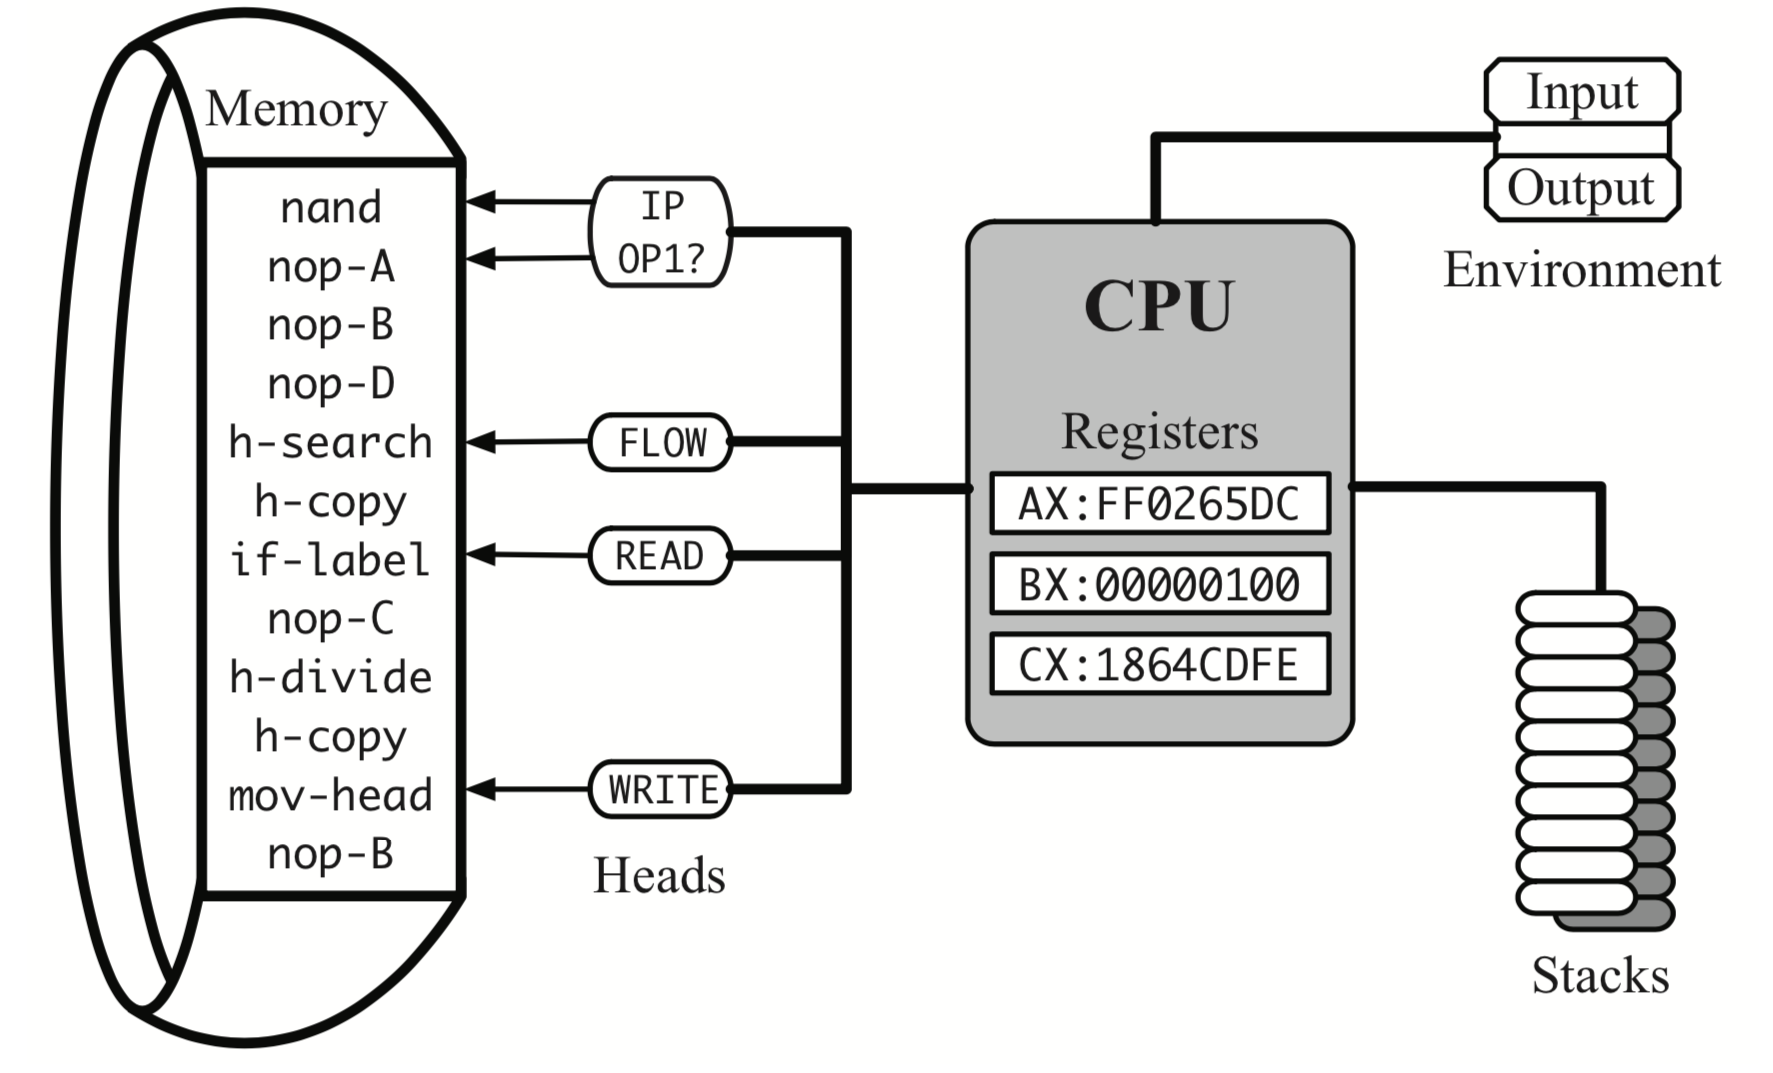
\includegraphics[width=\textwidth]{chapters/02-evolutionary-origins-of-plasticity/media/avida-virtual-cpu.png}
  \caption{\small 
    \textbf{A visual representation of the default virtual hardware used by organisms in Avida. }
    Original figure from \citep{ofria_avida:_2009}.
  }
  \label{chapter:origins-of-plasticity:fig:avida-virtual-cpu}
\end{figure*}

% Metabolism, competition
Organisms can gain additional CPU cycles by performing tasks---such as mathematical computations---to improve their metabolic rate. 
An organism's metabolic rate determines how rapidly it can execute its genome; a higher metabolic rate allows an organism to replicate faster. 
Initially, an organism's metabolic rate is roughly proportional to its genome length; however, the organism's metabolic rate can be adjusted when the organism completes a task. 
In this way, we can differentially reward or punish the performance of different tasks.

When an organism successfully replicates, its offspring is placed in a random location in the world, replacing the organism formerly occupying that location. 
In this way, becoming a more efficient replicator in Avida is advantageous in the competition for space. 
The combination of competition for replication efficiency and heritable variation due to imperfect copying during the replication process results in evolution by natural selection. 

\subsubsection{Sensing in Avida}
\label{chapter:origins-of-plasticity:sec:methods:avida:sensing}

% Sensing in Avida
In a typical Avida run, organisms must execute an instruction called \code{IO} to output the result of a computation. 
That output is analyzed to determine if any tasks have been performed, and if so, the organism is appropriately rewarded or punished. 
However, in this default scenario, organisms cannot sense the result, even after the task has been performed. 
To provide organisms with a mechanism to sense their environment, we added an \code{IO-Sense} instruction to the set of available instructions\footnote{
\code{IO-Sense} is based on the \code{IO-Feedback} instruction implemented in \citep{clune_investigating_2007}, which worked exactly as the default \code{IO} instruction, but provided the organism with feedback on the result.
As such, an organism must first do a particular task once---and potentially get punished---to sense whether or not the task is beneficial with the \code{IO-Feedback} instruction.
}.

The \code{IO-Sense} instruction simulates \code{IO} and provides the organism with feedback on what would have happened if the organism had executed an \code{IO} instruction instead. 
This separation of \code{IO} performance and sensing allows organisms to determine whether or not a particular task is being punished without the risk of punishment, lowering the potential cost of sensing. 
If an \code{IO} operation would have resulted in a punishment, a -1 is added to the top of the organism's stack memory; if it would have resulted in a reward, a 1 is placed there. 
If an \code{IO} operation would have resulted in neither a reward nor a punishment, a 0 is placed on the organism's stack memory. 
In this way, organisms can sense whether or not a particular task is being rewarded or punished in their current environment and then react accordingly.  

\subsubsection{Identifying Phenotypic Plasticity in Avida}
\label{chapter:origins-of-plasticity:sec:methods:avida:identifying-plasticity}

% identifying phenotypic plasticity in avida 
We define a phenotypically plastic organism in Avida as an organism that leverages sensory information to alter their phenotype based on the environment.
We restrict the definition of an organism's phenotype to the set of unique tasks it performs in the given environment. 
We do not consider how many times an organism performs a particular task in a given environment, but only whether the organism does the task at all. 
Thus, to be phenotypically plastic, an organism must express a different task profile (\textit{i.e.}, perform different tasks) in different environments. 

\subsection{Experimental Design}
\label{chapter:origins-of-plasticity:sec:methods:experimental-design}

% Lead-in
To explore the evolutionary history of phenotypically plastic organisms, we used an experimental design based on \citep{clune_investigating_2007}. 

% Environment
\subsubsection{Environments}
\label{chapter:origins-of-plasticity:sec:methods:experimental-design:environments}

We constructed two experimental environments named ENV-NAND and ENV-NOT.
In ENV-NAND, organisms were rewarded for performing the NAND logical task but were punished for performing the NOT logical task. 
Conversely, in ENV-NOT, organisms were rewarded for performing the NOT logical task but were punished for performing the NAND logical task. 
In each of our experimental treatments, we cycled between these two environmental conditions. 
In this way, genotypes with the capacity to sense the current environment and express the appropriate task had a competitive advantage over non-plastic organisms. 

\subsubsection{Phenotypes}
\label{chapter:origins-of-plasticity:sec:methods:experimental-design:phenotypes}

% Possible phenotypes
Given our simple definition of a phenotype, there are only four possible phenotypes in each of the two previously described environments: 
(1) perform only NAND, 
(2) perform only NOT, 
(3) perform both NAND and NOT, 
and (4) perform neither NAND nor NOT. 
When considering an organism's phenotype across both ENV-NAND and ENV-NOT, there are sixteen possible combinations. 
We enumerate these phenotypes in Figure \ref{chapter:origins-of-plasticity:fig:task-profiles}. 
Of these sixteen possible phenotypes, only four express the identical task profile in both environments; the other twelve profiles all exhibit some form of plasticity. 
The optimal form of plasticity is to perform only the NAND task in ENV-NAND and to perform only the NOT task in ENV-NOT; any other form of plasticity is sub-optimal. 
There are five possible phenotypes that leverage plasticity to perform punished tasks instead of rewarded tasks in a given environment; we did not expect these forms of phenotypic plasticity to be successful. 


% Table that enumerates possible phenotypic states
\begin{figure*}[!ht]
  \centering 
  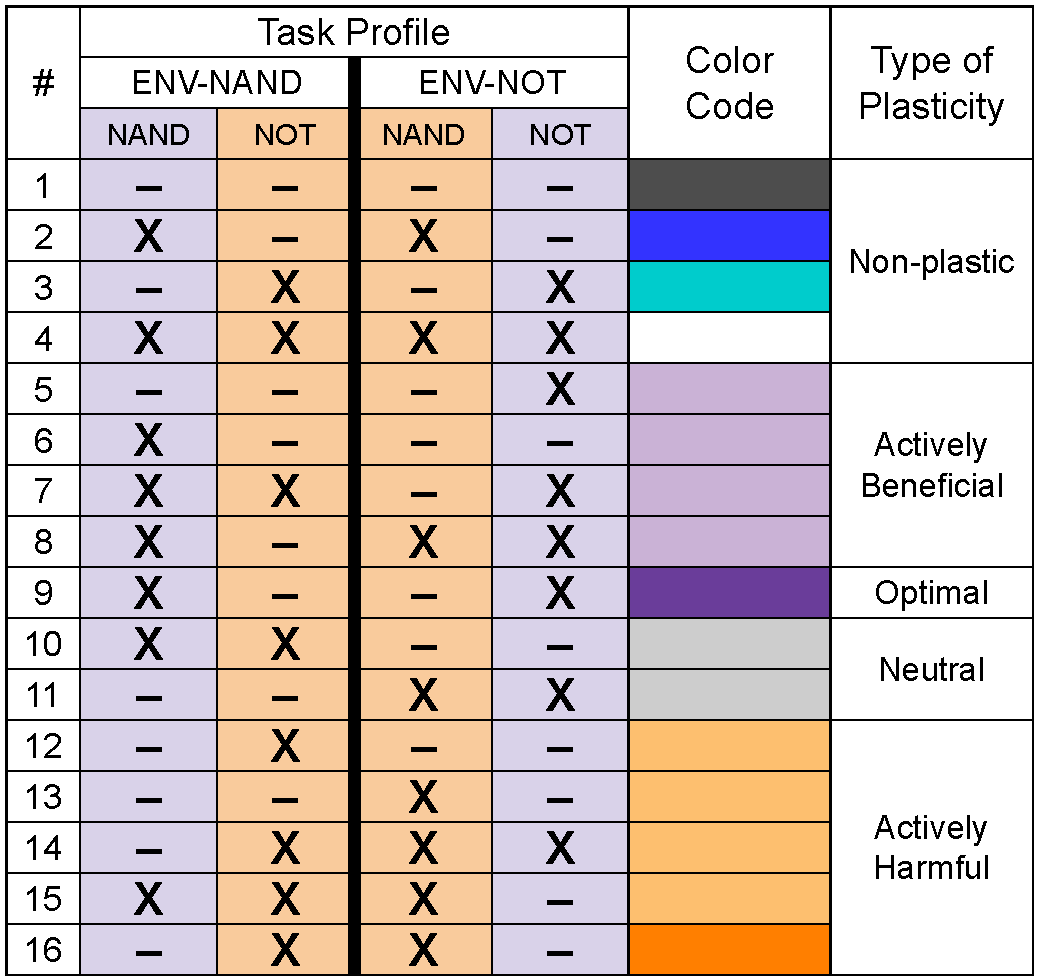
\includegraphics[width=0.75\columnwidth]{chapters/02-evolutionary-origins-of-plasticity/media/task-profiles.pdf}
  \caption{\small 
  \textbf{Enumeration of all possible complete phenotypes.}
  Each row represents a distinct phenotype. 
  An `X' indicates that the associated task is performed in the specified environment, while a `--' indicates that the task is not performed. 
  For each environment, the column of the rewarded task is highlighted in light purple, and the column of the punished task is highlighted in light orange. 
  An `X' in a reward column or a `--' in the punished column is optimal. 
  Each phenotype has a color code, which is used in our lineage visualization visualizations.  
  Note that the first four rows are non-plastic phenotypes, rows 5--8 exhibit partially beneficial plasticity, and row 9 is optimally beneficial.  
  Rows 10--11 are neutral non-adaptive plasticity, while rows 12--16 are detrimental forms of plasticity.}
  \label{chapter:origins-of-plasticity:fig:task-profiles}
\end{figure*}

\subsubsection{Treatments}
\label{chapter:origins-of-plasticity:sec:methods:experimental-design:treatments}

% Experimental treatments
Our experimental design consisted of five treatments and a control: 
(1) a baseline treatment with a moderate point-mutation rate and environmental-cycle length, 
(2) a low-mutation-rate treatment, 
(3) a high-mutation-rate treatment, 
(4) a short-environment-cycle-length treatment, 
(5) a long-environment-cycle-length treatment, 
and (6) a control where both NAND and NOT were rewarded and the environment did not fluctuate. 
See Table \ref{chapter:origins-of-plasticity:table:treatments} for treatment details.

We created the baseline treatment to produce phenotypically plastic organisms for lineage analysis. 
We limited the population size to 3600 organisms and seeded the world with an ancestral genotype capable only of self-replication.
We then evolved populations for 100,000 updates\footnote{
An update in Avida is an experimental length of time. One update is defined as the amount of time it takes for the average organism to execute 30 instructions (see \citep{ofria_avida:_2009} for more details).
} in Avida. 
We imposed a 0.0075 probability of point-mutation per instruction copied, as well as a 0.05 probability for each of single-instruction insertion and deletion per genome copied. 
We fluctuated the current environment between ENV-NAND and ENV-NOT every 100 updates in the baseline treatment. 
We ran 50 replicates of each treatment, including the control. 

% Table 'bout treatments
\begin{table}
\renewcommand{\arraystretch}{1.5}
  \centering
  \small
  \begin{tabular}{| >{\raggedright} p{0.3\columnwidth} |r | r| }
    \hline
    \centering \textbf{Treatment} & \multicolumn{1}{>{\raggedright\arraybackslash}p{0.25\columnwidth}|}{\centering \textbf{Point-mutation Rate}} & \multicolumn{1}{>{\raggedright\arraybackslash}p{0.30\columnwidth}|}{\centering \textbf{Environment Cycle Length }}
    \\ \hline 
    Baseline &  0.0075 &  100 updates  
    \\ \hline 
    Low Mutation Rate &  0.0025 & 100 updates 
    \\ \hline 
    High Mutation Rate &  0.0125 &  100 updates 
    \\ \hline
    Short Environment Cycle Length & 0.0075 &  50 updates 
    \\ \hline 
    Long Environment Cycle Length & 0.0075 &  200 updates 
    \\ \hline 
  \end{tabular}
  \caption{\small 
  \textbf{Differences among the five experimental treatments. }
  Point-mutation rate is given as mutations per instruction copied.
  Environment cycle length describes the length of time (in updates) an environment is active before toggling to the alternative environment.
  }
  \label{chapter:origins-of-plasticity:table:treatments}
\end{table}

\subsubsection{Lineage Visualization}
\label{chapter:origins-of-plasticity:sec:methods:experimental-design:lineage-visualization}

To explore evolutionary strategies evolved in fluctuating environments, we visualized the lineages of evolved genotypes as vertical bars where time (in updates) proceeds from top to bottom beginning with the lineage's original ancestor genotype.
Any given genotype on the lineage must express one of the sixteen possible phenotypes enumerated in Figure \ref{chapter:origins-of-plasticity:fig:task-profiles}.
At each point in time, the color of the visualized lineage corresponds to the color representing the phenotype expressed by the lineage at that point in time. 
For example, because the ancestral organism is capable only of self-replication, all visualized lineages should show that the original ancestor's phenotype performed neither the NAND task nor the NOT task. 
In addition to the visualized lineages, we indicate the actual environmental conditions experienced by the evolving populations at each point in time by the color of the vertical axis. 
This type of visualization allows us to display the phenotypic states traversed by any given lineage, allowing us to explore evolutionary strategies leveraged by all evolved lineages.
